\documentclass[border=10pt]{standalone}
\usepackage[svgnames]{xcolor}
\usepackage{amsmath}
\usepackage{pgfplots}
\pgfplotsset{compat=newest}
\usepackage[sfdefault]{FiraSans}
\usepackage{FiraMono}
\renewcommand*\familydefault{\sfdefault}
\begin{document}
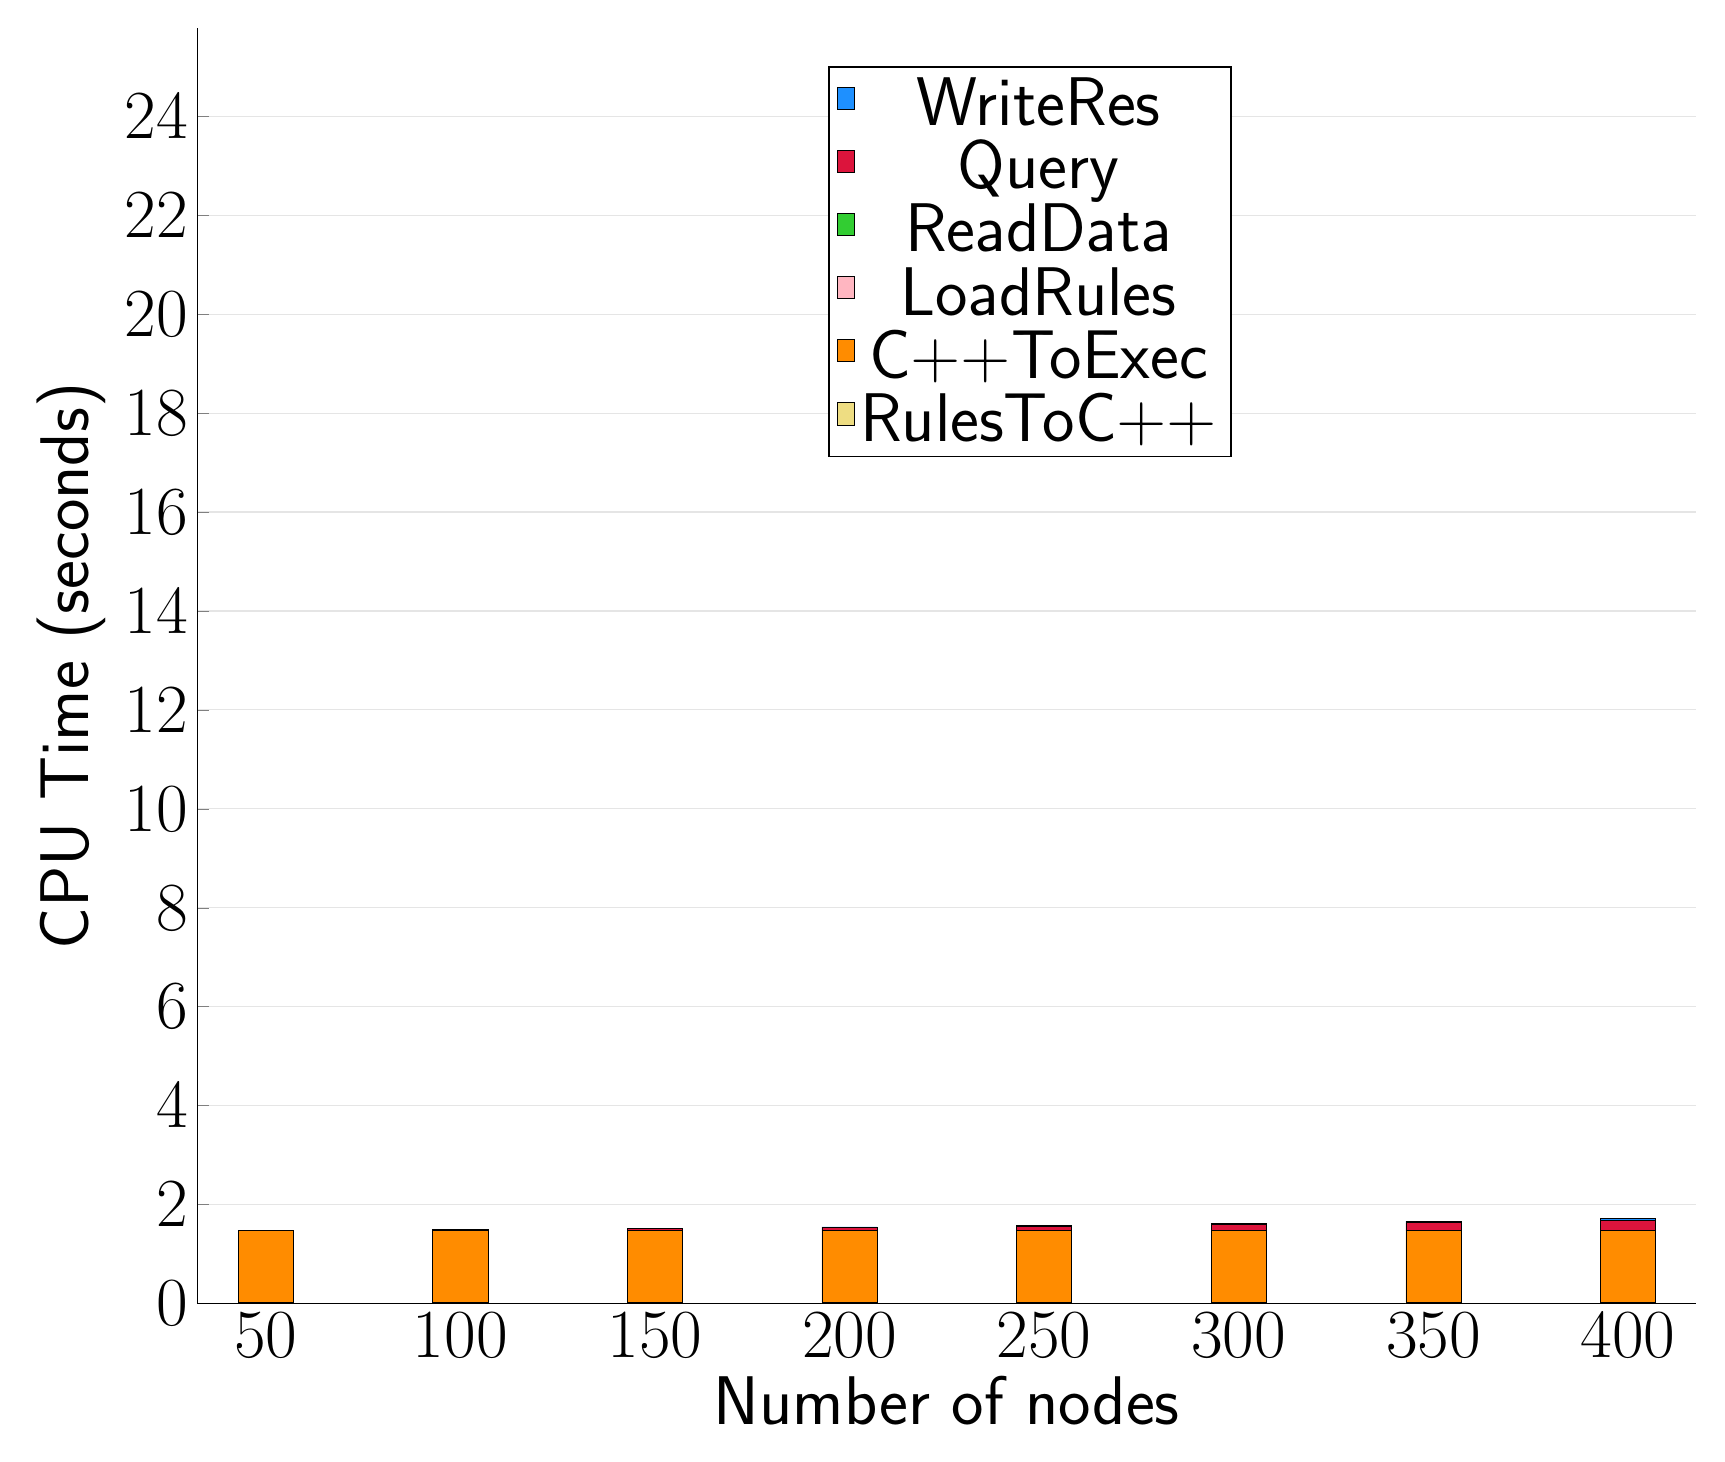
\begin{tikzpicture}
\begin{axis}[
   ybar stacked,
   width=1.7\textwidth,
   bar width=0.7cm,
   ymajorgrids, tick align=inside,
   major grid style={draw=gray!20},
   xtick=data,
   ymin=0, ymax=25.779619999999998,
   axis x line*=bottom,
   axis y line*=left,
   enlarge x limits=0.05,
   legend style={
       at={(0.69, 0.97)},
       anchor=north east,
       legend columns=1,
       font=\Huge,
   },
   ylabel={CPU Time (seconds)},
   xlabel={Number of nodes},
   label style={font=\Huge},
   tick label style={font=\Huge},
]
\addlegendimage{fill=DodgerBlue, draw=black, line width=0.2pt}
\addlegendentry{WriteRes}
\addlegendimage{fill=Crimson, draw=black, line width=0.2pt}
\addlegendentry{Query}
\addlegendimage{fill=LimeGreen, draw=black, line width=0.2pt}
\addlegendentry{ReadData}
\addlegendimage{fill=LightPink, draw=black, line width=0.2pt}
\addlegendentry{LoadRules}
\addlegendimage{fill=DarkOrange, draw=black, line width=0.2pt}
\addlegendentry{C++ToExec}
\addlegendimage{fill=LightGoldenrod, draw=black, line width=0.2pt}
\addlegendentry{RulesToC++}
\addplot +[fill=LightGoldenrod, draw=black, line width=0.2pt] coordinates {
(50, 0.031999999999999994)
(100, 0.030000000000000006)
(150, 0.030000000000000006)
(200, 0.030000000000000006)
(250, 0.030000000000000006)
(300, 0.030000000000000006)
(350, 0.030000000000000006)
(400, 0.030000000000000006)
};
\addplot +[fill=DarkOrange, draw=black, line width=0.2pt] coordinates {
(50, 1.448)
(100, 1.4469999999999996)
(150, 1.4469999999999998)
(200, 1.452)
(250, 1.448)
(300, 1.4509999999999998)
(350, 1.446)
(400, 1.4459999999999997)
};
\addplot +[fill=LightPink, draw=black, line width=0.2pt] coordinates {
(50, 7.48e-05)
(100, 9.85e-05)
(150, 0.0001135)
(200, 0.00010960000000000002)
(250, 8.34e-05)
(300, 0.00012580000000000002)
(350, 0.0001218)
(400, 0.0001245)
};
\addplot +[fill=LimeGreen, draw=black, line width=0.2pt] coordinates {
(50, 0.00030810000000000006)
(100, 0.0004485)
(150, 0.0006096)
(200, 0.0006659000000000001)
(250, 0.0007781)
(300, 0.0009249999999999999)
(350, 0.0010059000000000001)
(400, 0.0011401000000000002)
};
\addplot +[fill=Crimson, draw=black, line width=0.2pt] coordinates {
(50, 0.0040327)
(100, 0.0156366)
(150, 0.034923600000000006)
(200, 0.057228)
(250, 0.08456549999999999)
(300, 0.1179374)
(350, 0.15773580000000004)
(400, 0.20520049999999998)
};
\addplot +[fill=DodgerBlue, draw=black, line width=0.2pt] coordinates {
(50, 0.0013583)
(100, 0.0038955000000000005)
(150, 0.007509399999999999)
(200, 0.0114633)
(250, 0.017619199999999998)
(300, 0.025294900000000002)
(350, 0.0344206)
(400, 0.0450318)
};
\end{axis}
\end{tikzpicture}

\end{document}
